\documentclass[tikz,border=10pt]{standalone}
\usetikzlibrary{positioning, shapes}

\begin{document}

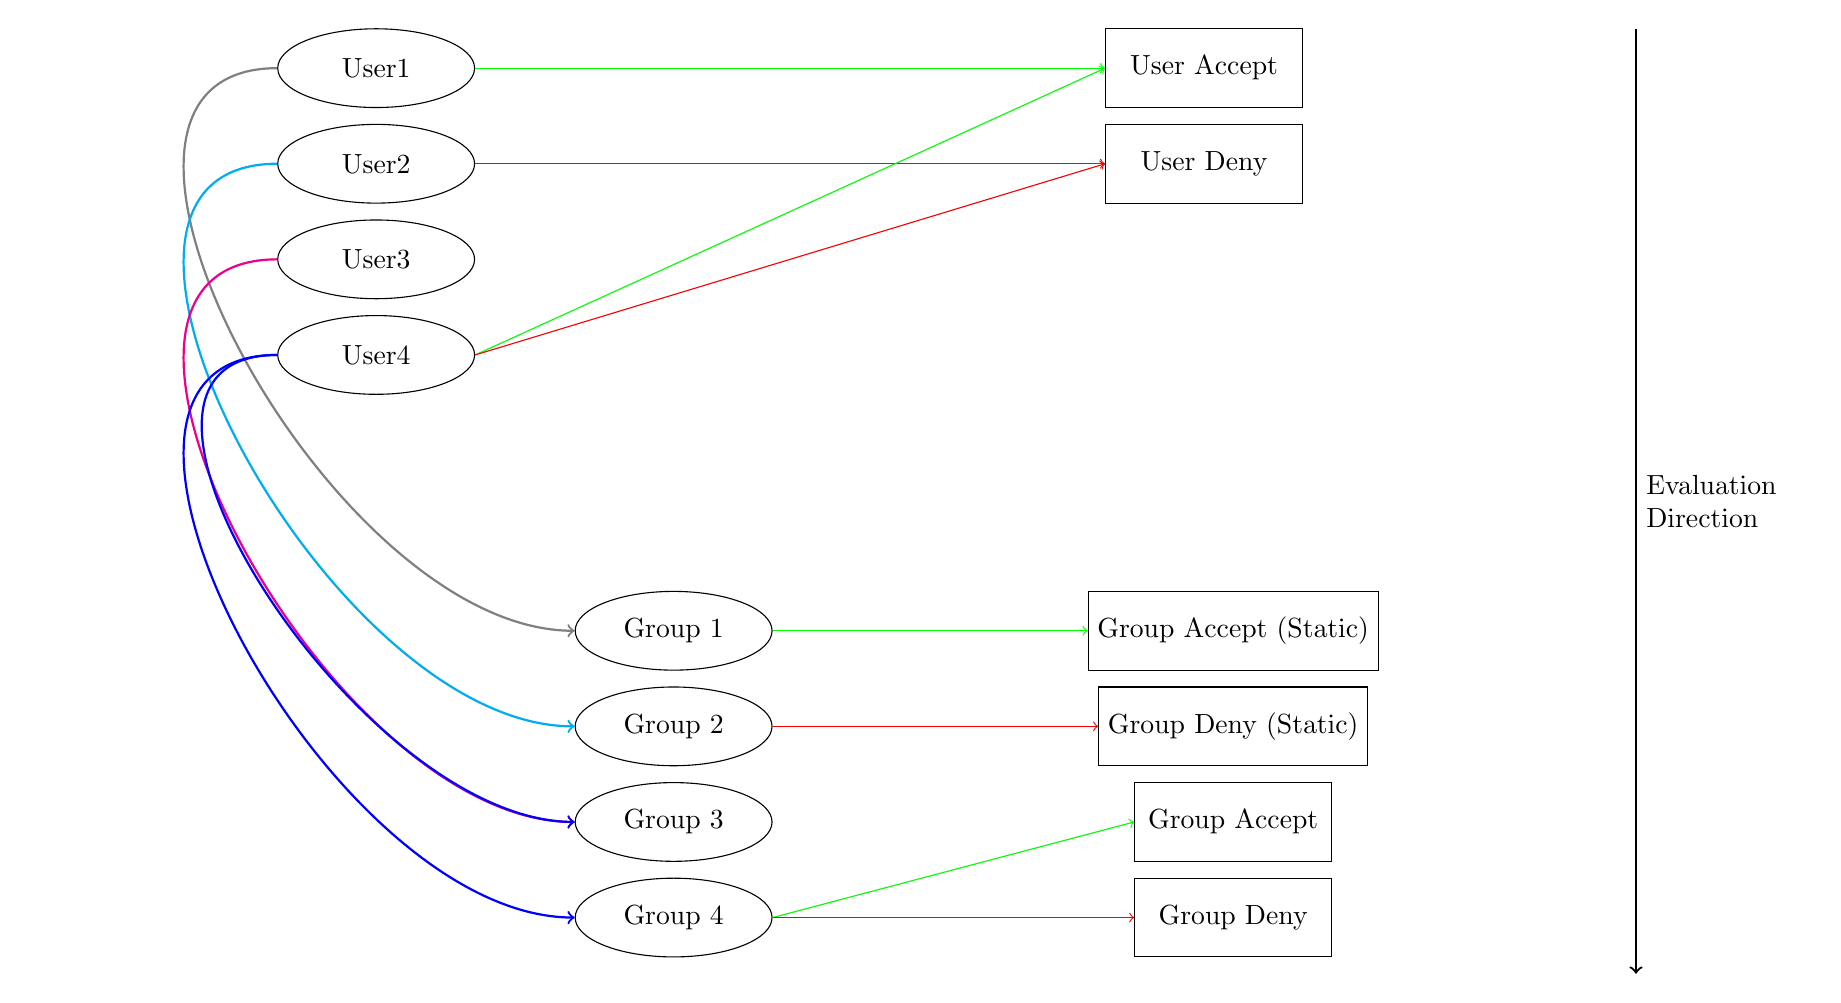
\begin{tikzpicture}[node distance=1.5cm]

% Users Column
\node[ellipse, draw, minimum width=2.5cm, minimum height=1cm] (user1) {User1};
\node[ellipse, draw, minimum width=2.5cm, minimum height=1cm, below=0.2cm of user1] (user2) {User2};
\node[ellipse, draw, minimum width=2.5cm, minimum height=1cm, below=0.2cm of user2] (user3) {User3};
\node[ellipse, draw, minimum width=2.5cm, minimum height=1cm, below=0.2cm of user3] (user4) {User4};

% User Rules Column
\node[draw, rectangle, minimum width=2.5cm, minimum height=1cm, right=8cm of user1] (user_accept) {User Accept};
\node[draw, rectangle, minimum width=2.5cm, minimum height=1cm, below=0.2cm of user_accept] (user_deny) {User Deny};

% Groups Column
\node[ellipse, draw, minimum width=2.5cm, minimum height=1cm, below right=4cm and 2cm of user3] (group1) {Group 1};
\node[ellipse, draw, minimum width=2.5cm, minimum height=1cm, below=0.2cm of group1] (group2) {Group 2};
\node[ellipse, draw, minimum width=2.5cm, minimum height=1cm, below=0.2cm of group2] (group3) {Group 3};
\node[ellipse, draw, minimum width=2.5cm, minimum height=1cm, below=0.2cm of group3] (group4) {Group 4};

% Group Rules Column
\node[draw, rectangle, minimum width=2.5cm, minimum height=1cm, right=4cm of group1] (group_static_accept) {Group Accept (Static)};
\node[draw, rectangle, minimum width=2.5cm, minimum height=1cm, below=0.2cm of group_static_accept] (group_static_deny) {Group Deny (Static)};
\node[draw, rectangle, minimum width=2.5cm, minimum height=1cm, below=0.2cm of group_static_deny] (group_accept) {Group Accept};
\node[draw, rectangle, minimum width=2.5cm, minimum height=1cm, below=0.2cm of group_accept] (group_deny) {Group Deny};

% Arrows
\draw[->, color=green] (user1.east) -- (user_accept.west);
\draw[->, color=red] (user2.east) -- (user_deny.west);
\draw[->, color=green] (user4.east) -- (user_accept.west);
\draw[->, color=red] (user4.east) -- (user_deny.west);

\draw[->, color=green] (group1.east) -- (group_static_accept.west);
\draw[->, color=red] (group2.east) -- (group_static_deny.west);
\draw[->, color=green] (group4.east) -- (group_accept.west);
\draw[->, color=red] (group4.east) -- (group_deny.west);


\draw[->,color=gray, thick] (user1.west) to[out=180, in=180] (group1.west);
\draw[->,color=cyan, thick] (user2.west) to[out=180, in=180] (group2.west);
\draw[->,color=magenta, thick] (user3.west) to[out=180, in=180] (group3.west);
\draw[->,color=blue, thick] (user4.west) to[out=180, in=180] (group3.west);
\draw[->,color=blue, thick] (user4.west) to[out=180, in=180] (group4.west);

% Evaluation Direction Arrow
\draw[->, thick] (16, 0.5) -- (16, -11.5) node[midway, right, text width=2cm] {Evaluation Direction};


\end{tikzpicture}

\end{document}
